\documentclass[12pt,compress,aspectratio=169]{beamer}
\usetheme{metropolis}
\setbeamersize{text margin left=.5cm,text margin right=.5cm}
\usepackage[lf]{carlito}
\usepackage{siunitx}
\usepackage{tikz}
\usepackage{mathpazo}
\usepackage{bm}
\usepackage{mathtools}
\usepackage[ISO]{diffcoeff}
\diffdef{}{ op-symbol=\mathsf{d} }
\usepackage{xcolor,colortbl}

\setmonofont{Ubuntu Mono}
\setlength{\parskip}{0pt}
\renewcommand{\baselinestretch}{1}

\sisetup{
  inter-unit-product=\cdot,
  per-mode=symbol
}

\tikzset{
  >=latex
}

%\newcommand{\iii}{\hat{\bm\imath}}
%\newcommand{\jjj}{\hat{\bm\jmath}}
%\newcommand{\kkk}{\hat{\bm k}}


\usetikzlibrary{decorations.pathmorphing,patterns}

\title{Class 2: Dynamics}
\subtitle{Advanced Placement Physics C}
\author[TML]{Dr.\ Timothy Leung}
\institute{Olympiads School}
\date{Updated: Summer 2022}

\newcommand{\pic}[2]{
  \includegraphics[width=#1\textwidth]{#2}
}
\newcommand{\eq}[2]{
  \vspace{#1}{\Large
    \begin{displaymath}
      #2
    \end{displaymath}
  }
}
%\newcommand{\iii}{\ensuremath\hat{\bm{\imath}}}
%\newcommand{\jjj}{\ensuremath\hat{\bm{\jmath}}}
%\newcommand{\kkk}{\ensuremath\hat{\bm{k}}}
\newcommand{\iii}{\ensuremath\hat\imath}
\newcommand{\jjj}{\ensuremath\hat\jmath}
\newcommand{\kkk}{\ensuremath\hat k}


\begin{document}

\begin{frame}
  \maketitle
\end{frame}



\begin{frame}{Dynamics}
  While \textbf{kinematics} describes the motion of any object mathematically,
  \textbf{dynamics} describes \emph{what} causes motion motion to change
\end{frame}



\section{Laws of Motion}

\begin{frame}{First Law of Motion}
  \begin{center}
    \fbox{
      \begin{minipage}{.66\textwidth}
        \textbf{First Law: Every object will remain in its state of rest or
          uniform motion, until a net external force is applied to it.}
      \end{minipage}
    }
  \end{center}
  \begin{itemize}
  \item Uniform motion means constant velocity; an object ``at rest'' is also
    in uniform motion with $\vec v=\vec 0$
  \item As long as an object moves in uniform motion, it must be that
    $\vec F_\text{net}=\vec 0$
  \item Common examples:
    \begin{itemize}
    \item A hockey puck sliding on very smooth ice has gravity and normal
      force, but the net force is zero
    \item A car traveling on a highway at \SI{100}{\kilo\metre\per\hour}
      has many forces acting on it, but the net force is zero 
    \end{itemize}
  \item\textcolor{red!80!black}{This is a special case that assumes a constant
    mass.}
  \end{itemize}
\end{frame}


\begin{frame}{Translational Equilibrium}
  If the net force on an object is zero ($\Sigma\vec F=\vec 0$) then the
  object is in a \emph{state of translational equilibrium}
  \begin{itemize}
  \item Dynamic equilibrium: the object is moving relative to us
  \item Static equilibrium: the object is not moving relative to us
  \end{itemize}
\end{frame}



\begin{frame}{Second Law of Motion}
  \begin{center}
    \fbox{
      \begin{minipage}{.68\textwidth}
        \textbf{Second Law: The acceleration of an object is proportional to,
          and along the direction of, the net external force.}
      \end{minipage}
    }
  \end{center}
  \begin{itemize}
  \item\textcolor{red!80!black}{Like the first law, this is also a
    ``special case'' that assumes a constant mass.}
  \item The first two laws of motion can be summarized in the equation:

    \eq{-.2in}{
      \boxed{\vec F_\text{net}=\Sigma\vec F=m\vec a}
    }
  \item For non-constant mass, net force is the rate of change of momentum
    $\vec p$:

    \eq{-.2in}{
      \boxed{
        \vec F_\text{net}=\diff{\vec p}t
      }
    }
  \end{itemize}
\end{frame}


\begin{frame}{Mass}
  What is \textbf{mass} then? It is
  \begin{itemize}
    \item the property of an object that relates its acceleration to the force
      applied to it. Literally, it means:

      \eq{-.2in}{
        m\equiv\frac{F_\text{net}}a
      }
    \item Intrinsic to the object itself
    \item This is explicitly referred to as the object's \textbf{inertial mass}
  \end{itemize}
\end{frame}



\begin{frame}{Third Law of Motion}
  \begin{center}
    \fbox{
      \begin{minipage}{.9\textwidth}
        \textbf{Third Law: For every action there is always and opposite and
          equal reaction; the mutual actions of two objects on each other are
          always equal, and directed to the other object.}
      \end{minipage}
    }
  \end{center}

  For every action force on an object (B) due to another object (A), there is a
  reaction force which is equal in magnitude but opposite in direction, on
  object (A), due to object (B):

  \eq{-.3in}{
    \boxed{\vec F_\text{AB} = -\vec F_\text{BA}}
  }
  \begin{itemize}
  \item The action and reaction forces act on different objects!
  \item Third law is the natural consequence of the first and second law.
    Action/reaction forces are \emph{internal} forces.
  \end{itemize}
  \vspace{.2in}
\end{frame}



\begin{frame}{Forces}
  A \textbf{force} is the interaction between the objects.
  \begin{itemize}
  \item When there is interaction, then forces are created
  \item A ``push'' or a ``pull''
  \end{itemize}
  There are two broad categories of forces:
  \begin{itemize}
  \item\textbf{Contact forces} act between two objects that are in contact
    with one another
  \item\textbf{Non-contact forces} act between two objects without them
    touching each other. They are also called ``action-at-a-distance'' force
  \end{itemize}
\end{frame}



\section{Common Forces}

\begin{frame}{Common Forces}
  Common forces that we encounter in AP Physics include:
  \begin{itemize}
  \item Weight (gravitational force) $\vec w$ (or $\vec F_g$, or just $m\vec g$)
  \item Normal force $\vec N$
  \item Friction (static $\vec f_s$ and kinetic $\vec f_k$)
  \item Tension $\vec T$
  \item Applied force $\vec F_a$
  \item Spring force $\vec F_e$
  \item Drag $\vec D$ (fluid resistance)
  \item Buoyant force $\vec D$ (discussed in fluid mechanics, in AP Physics 2)
  \item Electrostatic force $\vec F_q$ (discussed in E \& M)
  \item Magnetic force $\vec F_m$ (discussed E \& M)
  \end{itemize}
\end{frame}



\begin{frame}{Gravity}
  Gravity is the force of attraction between all objects with mass
    
  \eq{-.2in}{
    \boxed{\vec w=m\vec g}
  }
  \begin{itemize}
  \item\vspace{-.15in}Near surface of Earth, use
    $g=\SI{9.81}{\metre\per\second\squared}$ (or
    $g=\SI{10}{\metre\per\second\squared}$ for your AP exam)
  \item You may be asked to find the value of $g$ on some ``unknown planet''.
  \item $\vec w$ always points \emph{down} (the direction of $\vec w$ is how
    down is defined)
  \item Based on the law of universal gravitation:

    \eq{-.3in}{
      \boxed{F_g=\frac{Gm_1m_2}{r^2}}\;\;
      \text{\normalsize where}\;\;
      G=\SI{6.674e-11}{\newton\metre\squared\per\kilo\gram\squared}
    }
  \end{itemize}    
\end{frame}



\begin{frame}{Normal Force}
  \begin{columns}
    \column{.22\textwidth}
    \centering
    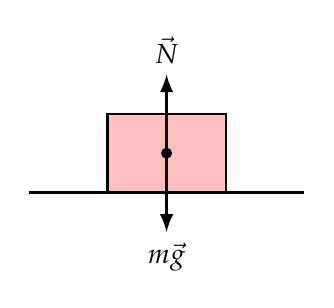
\begin{tikzpicture}{scale=1.5}
      \draw[thick] (-1,0)--(2.5,0);
      \draw[fill=pink,thick] rectangle (1.5,1);
      \fill(.75,.5) circle(2pt);
      \draw[->,very thick] (.75,.5)--(.75,-.5) node[below]{$m\vec g$};
      \draw[->,very thick] (.75,.5)--(.75,1.5) node[above]{$\vec N$};
    \end{tikzpicture}
    
    $m\vec g=-\vec N$\\(special case)
    
    \column{.78\textwidth}
    \begin{itemize}
    \item A force a surface exerts on another object that it is in contact with
    \item Always \textbf{perpendicular} to the contact surface
    \item\textbf{Special case:} When an object is on a horizontal surface
      with no additional applied force, the magnitude of the normal force is
      equal to the magnitude of the weight of the object, i.e.\ $N=mg$
    \end{itemize}
  \end{columns}
\end{frame}



\begin{frame}{Normal Force on a Stationary Slope}
  For this case, we define the $x$-axis to be along the slope, and $y$-axis to
  be perpendicular to the slope.
  \begin{columns}
    \column{.35\textwidth}
    \centering
    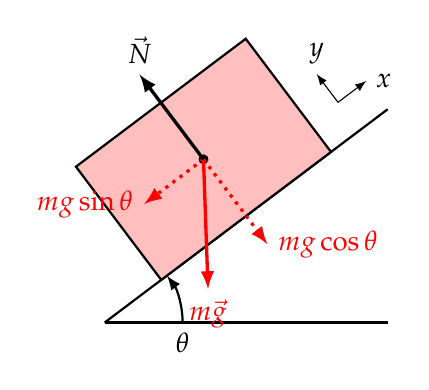
\begin{tikzpicture}[scale=.9]
      \draw[thick] (-1,0)--(3,0);
      \draw[thick,->](.1,0) arc(0:37:1.1) node[pos=0,below]{$\theta$};
      \begin{scope}[rotate around={37:(-1,0)}]
        \draw[->](3.5,.5)--(4,.5)  node[right]{$x$};
        \draw[->](3.5,.5)--(3.5,1) node[above]{$y$};
        \draw[thick] (-1,0)--(4,0);
        \draw[fill=pink,thick] rectangle (3,2);
        \fill(1.5,1) circle (2pt);
        \draw [->,very thick,dotted,red] (1.5,1)--(1.5,-.5)
        node[right]{$mg\cos\theta$};
        \draw [->,very thick,dotted,red] (1.5,1)--(.45,1)
        node[left]{$mg\sin\theta$};
        \draw [->,very thick,red] (1.5,1)--(.45,-.5)
        node[below]{$m\vec g$};
        \draw [->,very thick] (1.5,1)--(1.5,2.5) node[above]{$\vec N$};
      \end{scope}
    \end{tikzpicture}
    
    \column{.65\textwidth}
    \begin{itemize}
    \item On a stationary slope: $N=mg\cos\theta$
      \begin{itemize}
      \item $N$ decreases as ramp angle $\theta$ increases
      \end{itemize}
    \item Weight has a component along the ramp ($mg\sin\theta$) that wants
      to slide the block down.
    \end{itemize}
  \end{columns}
\end{frame}



\begin{frame}{Friction}
  \begin{itemize}
  \item A force that opposes the sliding of two surface against one another
  \item Always act in a direction that opposes motion or attempted motion
  \item Depends on:
    \begin{itemize}
    \item Normal force $N$: The force the two surfaces are pressed against
      each other
    \item Coefficient of friction ($\mu_s$ and $\mu_k$): Smoothness of the
      surfaces, which itself depends on
      \begin{itemize}
      \item The material(s) the surfaces are made of
      \item The use of lubricants
      \end{itemize}
    \end{itemize}
  \end{itemize}
  \begin{center}
    \vspace{-.1in}
    \pic{.5}{graphics/friction}
  \end{center}
\end{frame}



\begin{frame}{Static Friction}
  \textbf{Static friction} between the two surfaces is when there is no
  relative motion between them
  \begin{itemize}
  \item Increases with increasing applied force
  \item Maximum when the object is just about to move
  \end{itemize}

  \eq{-.35in}{
    \boxed{f_s\leq\mu_sN}
  }
  \begin{center}
    \begin{tabular}{l|c|c}
      \rowcolor{pink}
      \textbf{Quantity} & \textbf{Symbol} & \textbf{SI Unit} \\ \hline
      Magnitude of static friction & $f_s$ & \si\newton \\
      Static friction coefficient  & $\mu_s$ & no units \\
      Magnitude of normal force    & $N$ & \si\newton
    \end{tabular}
  \end{center}
\end{frame}



\begin{frame}{Kinetic Friction}
  \textbf{Kinetic friction} between two surfaces is when they are moving
  relative to each other. $f_k$ is constant along the path of movement as long
  as $\vec N$ stays constant

  \eq{-.3in}{
    \boxed{f_k = \mu_kN}
  }
  \begin{center}
    \begin{tabular}{l|c|c}
      \rowcolor{pink}
      \textbf{Quantity} & \textbf{Symbol} & \textbf{SI Unit} \\ \hline
      Magnitude of kinetic friction & $f_k$ & \si\newton \\
      Kinetic friction coefficient  & $\mu_k$ & no units \\
      Magnitude of normal force     & $N$ & \si\newton
    \end{tabular}
  \end{center}
\end{frame}



\begin{frame}{Static and Kinetic Coefficients of Friction}    
  Kinetic friction coefficient is always lower than the static coefficient,
  otherwise nothing will ever move:
    
  \eq{-.45in}{
    \mu_k\leq\mu_s
  }

  \vspace{-.2in}Consider a simple case of a box being pulled along a level
  floor. The free-body diagram is simple (left). How do the magnitudes of the
  applied force $F_a$ and friction $f$ compare?

  \vspace{-.2in}
  \begin{columns}
    \column{.4\textwidth}
    \centering
    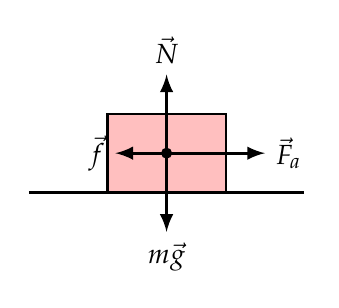
\begin{tikzpicture}
      \draw [thick] (-1,0)--(2.5,0);
      \draw [fill=pink,thick] rectangle (1.5,1);
      \fill (.75,.5) circle(2pt);
      \begin{scope}[->,very thick]
        \draw(.75,.5)--(.75,-.5) node[below]{$m\vec g$};
        \draw(.75,.5)--(.75,1.5) node[above]{$\vec N$};
        \draw(.75,.5)--(2.,.5)   node[right]{$\vec F_a$};
        \draw(.75,.5)--(.1,.5)   node[left] {$\vec f$};
      \end{scope}
    \end{tikzpicture}

    \column{.6\textwidth}
    \centering
    \begin{tikzpicture}[scale=.5]
      \draw[very thick,->](0,0)--(10,0) node[right]{$F_a$};
      \draw[very thick,->](0,0)--(0,5) node[left]{$f$};
    \end{tikzpicture}
  \end{columns}
\end{frame}



\begin{frame}{Tires}
  Most people associate friction as the force that slows down things, but very
  often friction is what accelerates things. \textbf{Example:} the forward
  acceleration of a car is caused by the static friction between the tires and
  the road.
  \begin{center}
    \pic{.38}{graphics/all-season-tires}
  \end{center}
  Tires also generated a force called \emph{rolling resistance} as it rolls
  along a road because the weight of the car deforms the tires.
\end{frame}




\begin{frame}{Drag}
  When an object moves through a fluid (most gases and liquids), it experiences
  are fluid resistance force called \textbf{drag} $\vec D$.
  \begin{center}
    \pic{.338}{graphics/boeing787}
    \pic{.35}{graphics/ganna}
    \pic{.263}{graphics/submarine}
  \end{center}
  Unlike kinetic friction, drag force is highly dependent on the speed of the
  object relative to the fluid that it is moving in:
  
  \eq{-.28in}{
    D=\frac12\rho v_\infty^2C_dA
  }

  \vspace{-.1in}In AP Physics you are \emph{not} asked to know the drag
  equation. However, you should know that drag depends on speed and is not a
  constant.
\end{frame}



\begin{frame}{Drag}
  \eq{-.1in}{
    \boxed{ D=\frac12\rho v_\infty^2C_dA }
  }  
  \begin{center}
    \begin{tabular}{l|c|c}
      \rowcolor{pink}
      \textbf{Quantity} & \textbf{Symbol} & \textbf{SI Unit} \\ \hline
      Magnitude of drag force & $D$       & \si\newton \\
      Density of the fluid    & $\rho$    & \si{\kilo\gram\per\metre\cubed}\\
      Free-stream velocity    & $v_\infty$ & \si{\metre\per\second}\\
      Reference area          & $A$       & \si{\metre\squared}\\
      Drag coefficient        & $C_d$     & (no unit)
    \end{tabular}
  \end{center}
  Drag coefficient depends on the shape and surface smoothness of the object.
  For blunt objects (``bluff bodies'') $A$ is the frontal area; for
  streamlined objects $A$ is the planform (top-view) area
\end{frame}



\begin{frame}{Terminal Velocity}
  When we take drag force into account, we understand that the drag force
  increases as an object speeds up, and therefore a free-falling object does
  \emph{not} accelerate infinitely. Instead it reaches a
  \textbf{terminal velocity}.

  \begin{columns}
    \column{.33\textwidth}
    
    {\footnotesize There is no air resistance just as the object \emph{begins}
      to fall. Acceleration is due to gravity alone.\par}

    \vspace{-.15in}
    \begin{center}
      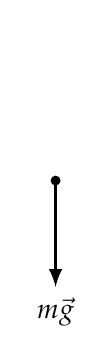
\begin{tikzpicture}[scale=.9]
        \draw[very thick,->](0,0)--(0,-1.5) node[below]{$m\vec g$};
        \draw[very thick,->,white](0,0)--(0,1.5) node[above]{$\vec D$};
        \fill circle(.07);
      \end{tikzpicture}
    \end{center}
    
    \column{.33\textwidth}

    {\footnotesize Drag increases as $v$ increases. Magnitude of acceleration
      decreases, but the object continues to gather speed\par}

    \vspace{-.15in}
    \begin{center}
      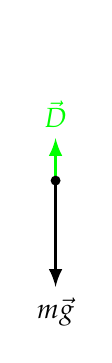
\begin{tikzpicture}[scale=.9]
        \draw[very thick,->](0,0)--(0,-1.5) node[below]{$m\vec g$};
        \draw[very thick,->,white](0,0)--(0,1.5) node[above]{$\vec D$};
        \draw[very thick,->,green](0,0)--(0,.6) node[above]{$\vec D$};
        \fill circle(.07);
      \end{tikzpicture}
    \end{center}
    
    \column{.33\textwidth}
    
    {\footnotesize Terminal velocity is reached when the drag force equals the
      object's weight. Not net force; no acceleration.\par}

    \vspace{-.15in}
    \begin{center}
      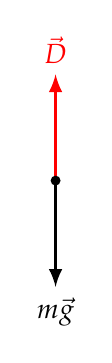
\begin{tikzpicture}[scale=.9]
        \draw[very thick,->](0,0)--(0,-1.5) node[below]{$m\vec g$};
        \draw[very thick,->,red](0,0)--(0,1.5) node[above]{$\vec D$};
        \fill circle(.07);
      \end{tikzpicture}
    \end{center}
        
  \end{columns}
\end{frame}




%\begin{frame}{Example Problem}
%  \textbf{Example 8:} To move a \SI{45}{kg} wooden crate across a wooden floor
%  ($\mu=0.20$), you tie a rope onto the crate and pull on the rope. While you
%  are pulling the rope with a force of \SI{115}{N}, it makes an angle of
%  \ang{15}
%  with the horizontal. How much time elapses between the time at which the
%  crate just starts to move and the time at which you are pulling it with a
%  velocity of \SI{1.4}{m/s}?
%  \begin{center}
%    \pic{.5}{graphics/pull-box}
%  \end{center}
%\end{frame}
%
%\begin{frame}{Example Problem}
%  \textbf{Example 9:} You are holding an \SI{85}{kg} trunk at the top of a ramp
%  that slopes from a moving van to the ground, making an angle of \ang{35} with
%  the ground. You lose your grip and the trunk begins to slide.
%  \begin{itemize}
%  \item If the coefficient of friction between the trunk and the ramp is
%    $0.42$, what is the acceleration of the trunk?
%  \item If the trunk slides \SI{1.3}{m} before reaching the bottom of the ramp,
%    for what time interval did it slide?
%  \end{itemize}
%\end{frame}
%
%\begin{frame}{Example: Vertical Motion}
%  \textbf{Example 10:} A \SI{55}{kg} person is standing on a scale in an
%  elevator. If
%  the scale is calibrated in \emph{newtons}, what is the reading on the scale
%  when the elevator is not moving? If the elevator begins to accelerate upward
%  at \SI{.75}{m/s^2}, what will be the reading on the scale?
%\end{frame}



\begin{frame}{Tension Force}
  \textbf{Tension} $\vec T$ is the force that is the force that is transmitted
  through objects that can be stretched, e.g.\ a rope that is being pulled
  \begin{center}
    \pic{.6}{graphics/3-rope}
  \end{center}
  \begin{itemize}
  \item Examples: ropes, cables, strings, etc.
  \item Tension force can only be transmitted if the cable is fully extended
  \item You can't push on a rope
  \item Can be used with pulleys to change the direction of force
  \end{itemize}
\end{frame}



\begin{frame}{Spring Force \& Elastic Potential Energy}
  The spring force $\vec F_e$ is the force that a compressed/stretched spring
  exerts on the object connected to it.  An \emph{ideal} spring obeys Hooke's
  law:
    
  \eq{-.2in}{
    \boxed{\vec F_e=-k\vec x}
  }

  \vspace{-.1in}The spring force acts in the opposite direction to the spring's
  displacement, and is proportional to the amount of compression/stretching.

  \vspace{.1in}
  \begin{center}
    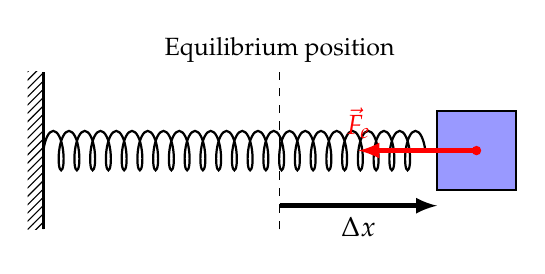
\begin{tikzpicture}
      \draw[thick,fill=blue!40] (5,.5) rectangle (6,1.5);
      \draw[thick,
        decoration={aspect=.3,segment length=2mm, amplitude=2.5mm, coil},
        decorate] (0,1)--(5,1);
      \fill[pattern=north east lines](-.2,0) rectangle(0,2);
      \draw[thick](0,.0)--(0,2);
      \fill[red] (5.5,1) circle(.06);
      \draw[ultra thick,->,red](5.5,1)--(4,1) node[above]{$\vec F_e$};
      \draw[dashed](3,0)--(3,2) node[above]{\small Equilibrium position};
      \draw[ultra thick,->](3,.3)--(5,.3) node[midway,below]{$\Delta x$};
    \end{tikzpicture}
    \hspace{.2in}
    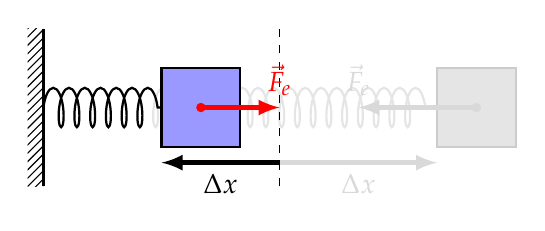
\begin{tikzpicture}
      \draw[thick,gray!40,fill=gray!20] (5,.5) rectangle (6,1.5);
      \draw[thick,gray!20,
        decoration={aspect=.3,segment length=2mm, amplitude=2.5mm, coil},
        decorate] (0,1)--(5,1);
      \fill[pattern=north east lines](-.2,0) rectangle(0,2);
      \draw[thick](0,.0)--(0,2);
      \fill[gray!30] (5.5,1) circle(.06);
      \draw[ultra thick,->,gray!30](5.5,1)--(4,1) node[above]{$\vec F_e$};
      \draw[dashed](3,0)--(3,2);
      \draw[ultra thick,->,gray!30](3,.3)--(5,.3)node[midway,below]{$\Delta x$};
      \draw[thick,fill=blue!40] (1.5,.5) rectangle (2.5,1.5);
      \draw[thick,
        decoration={aspect=.3,segment length=2mm, amplitude=2.5mm, coil},
        decorate] (0,1)--(1.5,1);
      \draw[ultra thick,->](3,.3)--(1.5,.3) node[midway,below]{$\Delta x$};
      \fill[red] (2,1) circle(.06);
      \draw[ultra thick,->,red](2,1)--(3,1) node[above]{$\vec F_e$};
    \end{tikzpicture}
  \end{center}
\end{frame}
%
%
%
%\begin{frame}{Spring Force}
%  The spring force $F_e$ is the force a compressed or stretched spring
%  exerts onto objects connected to it. It obeys Hooke's Law:
%  
%  \eq{-.2in}{
%    \vec F_s=-k\vec x
%  }
%  where $\vec x$ is the relative displacement of the ends of the spring.
%  \begin{center}
%    \pic{.35}{graphics/spring-example1}
%  \end{center}
%\end{frame}
%
%
%\begin{frame}{Spring Force}
%  \begin{center}
%    \pic{.28}{graphics/spring-example1}
%  \end{center}
%  \begin{itemize}
%  \item\vspace{-.15in}As the object falls onto the spring, the spring begins to
%    compress
%  \item As the spring compresses, the spring force (pointing up!) increases
%    linearly (Hooke's law)
%  \item At some point, the spring force balances the weight of the block
%    \begin{itemize}
%    \item At this point, the \emph{acceleration} is zero
%    \item But the velocity continues to be downward
%    \end{itemize}
%  \item The spring continues to compress until velocity is zero
%  \end{itemize}
%\end{frame}
%
%
%
%\begin{frame}{Spring Force}
%  \begin{center}
%    \pic{.28}{graphics/spring-example1}
%  \end{center}
%  \begin{itemize}
%  \item\vspace{-.15in}Solving this problem using dynamics is difficult, because:
%    \begin{itemize}
%    \item Spring force scales linearly with \emph{displacement}, but
%    \item Net force scales linearly with \emph{acceleration} (2nd time
%      derivative of displacement)
%    \end{itemize}
%  \item Note that the block continues to \emph{increase} velocity even after
%    it starts to compress the spring.
%  \item Acceleration is zero only after the spring has compressed some amount
%  \end{itemize}
%\end{frame}



%\begin{frame}{Buoyancy}{Everything Floats a Little}
%  When an object is submerged inside a fluid (e.g.\ water, air, etc), the fluid
%  exerts a pressure at the surface of the object. We can integrate the pressure
%  over the entire surface area $S$ to find the total force $\vec B$ the fluid
%  exerts on the object.
%  \begin{center}
%    \pic{.25}{graphics/rock_fbvectors}
%  \end{center}
%\end{frame}
%
%
%
%\begin{frame}{Buoyancy}
%  \framesubtitle{Everything Floats a Little}
%  The buoyant force is given by:
%  
%  \eq{-.1in}{
%    \vec{B}
%    =\rho_\text{fluid}g\vec{\hat{k}}\iiint dV
%    =\rho_\text{fluid}gV\vec{\hat{k}}
%  }
%  \begin{center}
%    \begin{tabular}{l|c|c}
%      \rowcolor{pink}
%      \textbf{Quantity} & \textbf{Symbol} & \textbf{SI Unit} \\ \hline
%      Buoyant force & $\vec{B}$  & \si{\newton} \\
%      Density of the fluid & $\rho_\text{fluid}$ & \si{\kg/\m^3}\\
%      Volume of the object & $V$ & \si{\metre^3}
%    \end{tabular}
%  \end{center}
%
%  We will discuss this later in the course, when we deal with fluid mechanics.
%\end{frame}



\section{Free-Body Diagrams}

\begin{frame}{Free-Body Diagrams}
  \begin{itemize}
  \item Acceleration (if there is going to be any at all) depends
    on net force $\vec F_\text{net}$
  \item Without a vector sum of all the forces, we cannot determine the
    magnitude, direction of the acceleration, or how acceleration will evolve
    in time
  \item We use \textbf{free-body diagrams} (FBD) to represent all the forces.
    \begin{itemize}
    \item Very important in solving any dynamics problems
    \item Don't try to save this step, even if the problem does not ask for it
    \item Always draw FBD for solving classical mechanics problem
    \end{itemize}
  \end{itemize}
\end{frame}



\begin{frame}{Free-Body Diagrams}
  For \emph{rectilinear}, or \emph{translational} motion, FBDs are usually drawn
  by assuming that all forces acting at the center of mass (``CM''),
  represented by the ``big dot''. For example:
  \begin{center}
    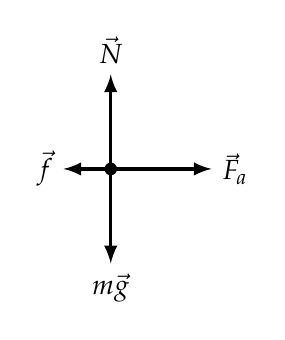
\begin{tikzpicture}[scale=.8]
      \fill(1.5,1) circle(.1);
      \begin{scope}[->,very thick]
        \draw(1.5,1)--(1.5,-.5) node[below]{$m\vec g$};
        \draw(1.5,1)--(1.5,2.5) node[above]{$\vec N$};
        \draw(1.5,1)--(3.1,1)   node[right]{$\vec F_a$};
        \draw(1.5,1)--(.75,1)   node[left] {$\vec f$};
      \end{scope}
    \end{tikzpicture}
  \end{center}
  However, for motion where \emph{rotation} is (at least) a possibility, we
  mist note that:
  \begin{itemize}
  \item Gravitational force $m\vec g$ acts at the CM, but
  \item Normal force $\vec N$, friction $\vec f$ and applied force $\vec F_a$
    act at the point of contact
  \end{itemize}
\end{frame}



\begin{frame}{Free-Body Diagrams}
  In those cases, forces should be drawn where they are applied. For example, a
  sphere rolling down a ramp should have weight $m\vec g$, normal force $\vec N$
  and static friction $\vec f_s$ acting on it:
  \begin{center}
    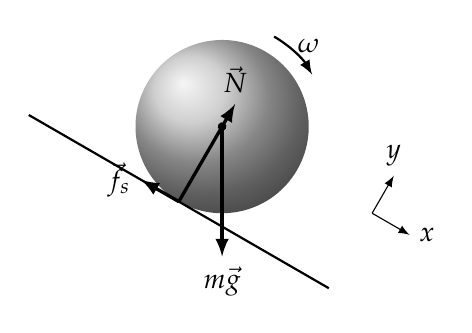
\begin{tikzpicture}[scale=1.1]
      \begin{scope}[rotate=-30]
	    \shade[ball color=gray!50] circle(1);
	    \draw[thick](-2,-1)--(2,-1);
	    \draw[thick,->](0,1.2) arc(90:60:1.2) node[pos=.3,right]{$\omega$};
	    \fill circle(.05);
	    \draw[->,very thick,rotate=30](0,0)--(0,-1.5)
	    node[below]{$m\vec g$};
	    \draw[->,very thick](0,-1)--(0,.3)  node[above]{$\vec N$};
	    \draw[->,very thick](0,-1)--(-.5,-1) node[left]{$\vec f_s$};
	    \draw[->](2,0)--(2.5,0) node[right]{$x$};
            \draw[->](2,0)--(2,.5) node[above]{$y$};
	  \end{scope}
	\end{tikzpicture}
  \end{center}
  Once the FBD is drawn, decide on the axes to help you solve the motion. One of
  the axes should line up with the direction of motion. This guarantees that
  the \emph{other} axis will not have any net force.
\end{frame}



\begin{frame}{Example Problem}
  A more difficult static problem may involve two surfaces with two different
  friction coefficients. For example, a ladder leaning on a wall. This problem
  cannot be solved without first understanding rotational motion, but we can
  still draw a FBD.
  \vspace{.2in}
  \begin{columns}
    \column{.75\textwidth}
    \textbf{Example:} A uniform ladder is \SI5{\metre} long and weighs
    \SI{400}\newton. The ladder rests against a slippery vertical wall, as
    shown in Figure. The inclination angle between the ladder and the rough
    floor is \ang{53}. Find the reaction forces from the floor and
    from the wall on the ladder and the coefficient of static friction $\mu_s$
    at the interface of the ladder with the floor that prevents the ladder from
    slipping.

    \column{.25\textwidth}
    \pic1{graphics/ladder}
  \end{columns}
\end{frame}



\section{Multi-Body Problems}

\begin{frame}{Applying Third Law on Connected Bodies}
  \begin{center}
    \pic{.7}{graphics/worldslongestroadtrainwithpowertrailer8}
  \end{center}
  \begin{itemize}
  \item The objects are connected by a cable or a solid linkage with negligible
    mass
  \item All objects (usually) have the same acceleration
  \item Require multiple free-body diagrams
  \end{itemize}
\end{frame}



\begin{frame}{Solving Connected-Bodies Problems}
  To solve a connected-bodies problem, you can follow these procedures:
  \begin{enumerate}
  \item Draw a FBD on each of the objects
  \item Sum all the forces on all the objects along the direction of motion
    \begin{itemize}
    \item Direction of motion is usually very obvious
    \item All internal forces should cancel and do not figure into the
      acceleration of the system
    \end{itemize}
  \item Compute the acceleration of the entire system using second law of motion
    \begin{itemize}
    \item Remember that (usually) every object has the same acceleration!
    \end{itemize}
  \item Go back to the FBD of each of the objects and compute the unknown
    forces (usually tension)
  \end{enumerate}
\end{frame}



%\begin{frame}{Connected Bodies: Example}
%  \textbf{Example:} A tractor-trailer pulling two trailers starts from rest
%  and accelerates with an acceleration $a$ on a straight, level road. The mass
%  of the truck (T) is \SI{5450}{\kilo\gram}, the mass of the first trailer (A)
%  is \SI{31500}{\kilo\gram}, and the mass of the second trailer (B) is
%  \SI{19600}{\kilo\gram}.
%  \begin{enumerate}
%  \item What magnitude of force must the truck generate in order to accelerate
%    the entire vehicle?
%  \item What magnitude of force must each of the trailer hitches withstand
%    while the vehicle is accelerating?
%  \end{enumerate}
%  Assume that frictional forces are negligible in comparison with the forces
%  needed to accelerate the large masses.
%\end{frame}


\begin{frame}{Different Types of Connected Bodies}
  Multiple objects pressed against one another. There may not be friction, but
  there are definitely action/reaction forces between the blocks.
  \begin{center}
    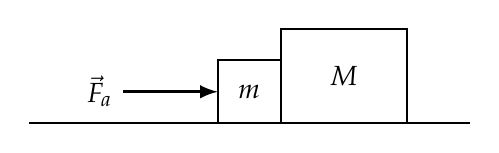
\begin{tikzpicture}[scale=.8]
      \begin{scope}[thick]
        \draw(-3,0)--(4,0);
        \draw rectangle(1,1)   node[midway]{$m$};
        \draw(1,0) rectangle(3,1.5) node[midway]{$M$};
      \end{scope}
      \draw[very thick,->](-1.5,.5)--(0,.5) node[pos=0,left]{$\vec F_a$};
    \end{tikzpicture}
  \end{center}
  Or multiple objects stacked on top of one another. The contact surface between
  $M$ and the floor may (or may not) have friction, while the surface between
  $M$ and $m$ must have a friction coefficient $\mu$.
  \begin{center}
    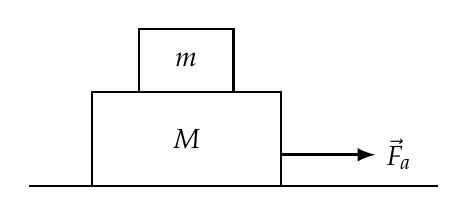
\begin{tikzpicture}[scale=.8]
      \begin{scope}[thick]
        \draw(-1,0)--(5.5,0);
        \draw rectangle(3,1.5) node[midway]{$M$};
        \draw(.75,1.5) rectangle(2.25,2.5) node[midway]{$m$};
      \end{scope}
      \draw[very thick,->](3,.5)--(4.5,.5) node[right]{$\vec F_a$};
    \end{tikzpicture}
  \end{center}
\end{frame}


\section{Pulley Problems}

\begin{frame}{Example Problem: Atwood Machine}
  An \textbf{Atwood machine} is made of two objects connected by a rope that
  runs over a pulley. The pulley allows the direction of force and direction
  of motion to change between two objects.
  \begin{columns}
    \column{.35\textwidth}
    \centering
    \pic1{graphics/pulley_prob_2}

    \column{.65\textwidth}
    \textbf{Example:} The object on the left has a mass of $M$ and the object
    on the right has a mass of $m$.
    \begin{itemize}
    \item What is the acceleration of the masses?
    \item What is the tension in the rope?
    \end{itemize}
  \end{columns}
\end{frame}


%\begin{frame}{A Difficult Problem!}
%  \begin{columns}
%    \column{.6\textwidth}
%    \textbf{Example:} Two blocks of mass $m$ and $M$ are connected via pulley
%    with a configuration as shown on the right. The coefficient of static
%    friction between the left block and the surface is $\mu_{s,1}$, and the
%    coefficient of static friction between the right block and the surface is
%    $\mu_{s,2}$. Formulate a mathematical inequality for the condition that no
%    sliding occurs. There may be more than one inequality. 
%    
%    \column{.4\textwidth}
%    \pic{1}{graphics/pulley_prob_6}
%  \end{columns}
%\end{frame}
%
%
%
%\begin{frame}{Multiple Pulleys}
%  When there are multiple pulleys involved, we have to remember that tension
%  force is distributed evenly along the cable.
%
%  \vspace{.2in}
%  \begin{columns}
%    \column{.6\textwidth}
%    \textbf{Example:} A block of mass $m$ is pulled, via two pulleys as shown,
%    at constant velocity along a surface inclined at angle $\theta$. The
%    coefficient of kinetic friction is $\mu_k$, between block and surface.
%    Determine the pulling force $F$. Ignore the mass of the pulleys. 
%    
%    \column{.4\textwidth}
%    \pic{1}{graphics/pulley_prob_7}
%  \end{columns}  
%\end{frame}


%\begin{frame}{One More!}
%  \begin{columns}
%    \column{.75\textwidth}
%    \textbf{Example:} A block of mass $M$ is lifted at constant velocity, via
%    an arrangement of pulleys as shown. Determine the pulling force $F$. Ignore
%    the mass of the pulleys. 
%
%    \uncover<2>{
%      \vspace{.2in}\textbf{Example:} The pulling force is replaced by a $10M$
%      mass, and was let go. What are the accelerations of the $M$ and the
%      $10M$ mass?
%    }
%    
%    \column{.25\textwidth}
%    \pic{1}{graphics/pulley_prob_9}
%  \end{columns}
%\end{frame}


\begin{frame}{A More Typical Problem}
  More typically, an Atwood machine problem is one where two objects are
  sliding on a surface. These surfaces may have (or may not) have friction. In
  this example, two blocks are connected by a massless string over a
  frictionless pulley as shown in the diagram.
  \begin{center}
    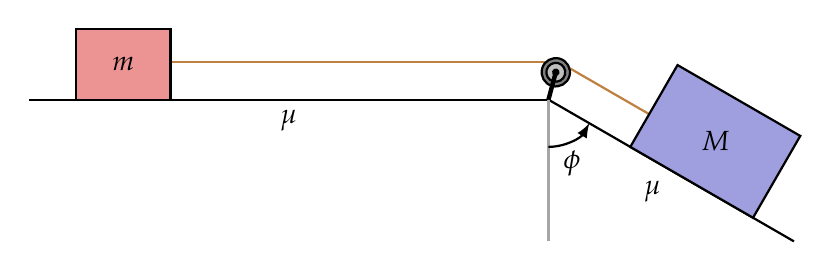
\begin{tikzpicture}[scale=1.2]
      \draw[thick,brown](-4,.4)--(.1,.4);
      \draw[thick](0,0)--(-5.5,0) node[midway,below]{$\mu$};
      \draw[thick,fill=red!70!gray!50](-4,0) rectangle(-5,.75)node[midway]{$m$};
      \begin{scope}[rotate=-30,thick]
        \draw[brown](1,.4)--(-.05,.4);
        \draw(0,0)--(3,0) node[midway,below left] {$\mu$};
        \draw[fill=blue!50!gray!50](1,0) rectangle(2.5,1)node[midway]{$M$};
      \end{scope}
      \begin{scope}[rotate=-15]
        \draw[thick,fill=gray] (0,.3) circle(.15);
        \draw[thick,fill=gray!50] (0,.3) circle(.1);
        \draw[ultra thick] (0,0)--(0,.3);
        \fill(0,.3) circle(.04);
      \end{scope}
      \draw[thick,gray!70](0,0)--(0,-1.5);
      \draw[thick,->](0,-.5)arc(270:330:.5) node[midway,below]{$\phi$};
    \end{tikzpicture}
  \end{center}
  \begin{enumerate}[(a)]
  \item Determine the acceleration of the blocks.
  \item Calculate the tension in the string.
  \end{enumerate}
\end{frame}
\end{document}
